% Options for packages loaded elsewhere
\PassOptionsToPackage{unicode}{hyperref}
\PassOptionsToPackage{hyphens}{url}
\PassOptionsToPackage{dvipsnames,svgnames,x11names}{xcolor}
%
\documentclass[
  letterpaper,
  DIV=11,
  numbers=noendperiod]{scrartcl}

\usepackage{amsmath,amssymb}
\usepackage{iftex}
\ifPDFTeX
  \usepackage[T1]{fontenc}
  \usepackage[utf8]{inputenc}
  \usepackage{textcomp} % provide euro and other symbols
\else % if luatex or xetex
  \usepackage{unicode-math}
  \defaultfontfeatures{Scale=MatchLowercase}
  \defaultfontfeatures[\rmfamily]{Ligatures=TeX,Scale=1}
\fi
\usepackage{lmodern}
\ifPDFTeX\else  
    % xetex/luatex font selection
\fi
% Use upquote if available, for straight quotes in verbatim environments
\IfFileExists{upquote.sty}{\usepackage{upquote}}{}
\IfFileExists{microtype.sty}{% use microtype if available
  \usepackage[]{microtype}
  \UseMicrotypeSet[protrusion]{basicmath} % disable protrusion for tt fonts
}{}
\makeatletter
\@ifundefined{KOMAClassName}{% if non-KOMA class
  \IfFileExists{parskip.sty}{%
    \usepackage{parskip}
  }{% else
    \setlength{\parindent}{0pt}
    \setlength{\parskip}{6pt plus 2pt minus 1pt}}
}{% if KOMA class
  \KOMAoptions{parskip=half}}
\makeatother
\usepackage{xcolor}
\setlength{\emergencystretch}{3em} % prevent overfull lines
\setcounter{secnumdepth}{5}
% Make \paragraph and \subparagraph free-standing
\makeatletter
\ifx\paragraph\undefined\else
  \let\oldparagraph\paragraph
  \renewcommand{\paragraph}{
    \@ifstar
      \xxxParagraphStar
      \xxxParagraphNoStar
  }
  \newcommand{\xxxParagraphStar}[1]{\oldparagraph*{#1}\mbox{}}
  \newcommand{\xxxParagraphNoStar}[1]{\oldparagraph{#1}\mbox{}}
\fi
\ifx\subparagraph\undefined\else
  \let\oldsubparagraph\subparagraph
  \renewcommand{\subparagraph}{
    \@ifstar
      \xxxSubParagraphStar
      \xxxSubParagraphNoStar
  }
  \newcommand{\xxxSubParagraphStar}[1]{\oldsubparagraph*{#1}\mbox{}}
  \newcommand{\xxxSubParagraphNoStar}[1]{\oldsubparagraph{#1}\mbox{}}
\fi
\makeatother

\usepackage{color}
\usepackage{fancyvrb}
\newcommand{\VerbBar}{|}
\newcommand{\VERB}{\Verb[commandchars=\\\{\}]}
\DefineVerbatimEnvironment{Highlighting}{Verbatim}{commandchars=\\\{\}}
% Add ',fontsize=\small' for more characters per line
\usepackage{framed}
\definecolor{shadecolor}{RGB}{241,243,245}
\newenvironment{Shaded}{\begin{snugshade}}{\end{snugshade}}
\newcommand{\AlertTok}[1]{\textcolor[rgb]{0.68,0.00,0.00}{#1}}
\newcommand{\AnnotationTok}[1]{\textcolor[rgb]{0.37,0.37,0.37}{#1}}
\newcommand{\AttributeTok}[1]{\textcolor[rgb]{0.40,0.45,0.13}{#1}}
\newcommand{\BaseNTok}[1]{\textcolor[rgb]{0.68,0.00,0.00}{#1}}
\newcommand{\BuiltInTok}[1]{\textcolor[rgb]{0.00,0.23,0.31}{#1}}
\newcommand{\CharTok}[1]{\textcolor[rgb]{0.13,0.47,0.30}{#1}}
\newcommand{\CommentTok}[1]{\textcolor[rgb]{0.37,0.37,0.37}{#1}}
\newcommand{\CommentVarTok}[1]{\textcolor[rgb]{0.37,0.37,0.37}{\textit{#1}}}
\newcommand{\ConstantTok}[1]{\textcolor[rgb]{0.56,0.35,0.01}{#1}}
\newcommand{\ControlFlowTok}[1]{\textcolor[rgb]{0.00,0.23,0.31}{\textbf{#1}}}
\newcommand{\DataTypeTok}[1]{\textcolor[rgb]{0.68,0.00,0.00}{#1}}
\newcommand{\DecValTok}[1]{\textcolor[rgb]{0.68,0.00,0.00}{#1}}
\newcommand{\DocumentationTok}[1]{\textcolor[rgb]{0.37,0.37,0.37}{\textit{#1}}}
\newcommand{\ErrorTok}[1]{\textcolor[rgb]{0.68,0.00,0.00}{#1}}
\newcommand{\ExtensionTok}[1]{\textcolor[rgb]{0.00,0.23,0.31}{#1}}
\newcommand{\FloatTok}[1]{\textcolor[rgb]{0.68,0.00,0.00}{#1}}
\newcommand{\FunctionTok}[1]{\textcolor[rgb]{0.28,0.35,0.67}{#1}}
\newcommand{\ImportTok}[1]{\textcolor[rgb]{0.00,0.46,0.62}{#1}}
\newcommand{\InformationTok}[1]{\textcolor[rgb]{0.37,0.37,0.37}{#1}}
\newcommand{\KeywordTok}[1]{\textcolor[rgb]{0.00,0.23,0.31}{\textbf{#1}}}
\newcommand{\NormalTok}[1]{\textcolor[rgb]{0.00,0.23,0.31}{#1}}
\newcommand{\OperatorTok}[1]{\textcolor[rgb]{0.37,0.37,0.37}{#1}}
\newcommand{\OtherTok}[1]{\textcolor[rgb]{0.00,0.23,0.31}{#1}}
\newcommand{\PreprocessorTok}[1]{\textcolor[rgb]{0.68,0.00,0.00}{#1}}
\newcommand{\RegionMarkerTok}[1]{\textcolor[rgb]{0.00,0.23,0.31}{#1}}
\newcommand{\SpecialCharTok}[1]{\textcolor[rgb]{0.37,0.37,0.37}{#1}}
\newcommand{\SpecialStringTok}[1]{\textcolor[rgb]{0.13,0.47,0.30}{#1}}
\newcommand{\StringTok}[1]{\textcolor[rgb]{0.13,0.47,0.30}{#1}}
\newcommand{\VariableTok}[1]{\textcolor[rgb]{0.07,0.07,0.07}{#1}}
\newcommand{\VerbatimStringTok}[1]{\textcolor[rgb]{0.13,0.47,0.30}{#1}}
\newcommand{\WarningTok}[1]{\textcolor[rgb]{0.37,0.37,0.37}{\textit{#1}}}

\providecommand{\tightlist}{%
  \setlength{\itemsep}{0pt}\setlength{\parskip}{0pt}}\usepackage{longtable,booktabs,array}
\usepackage{calc} % for calculating minipage widths
% Correct order of tables after \paragraph or \subparagraph
\usepackage{etoolbox}
\makeatletter
\patchcmd\longtable{\par}{\if@noskipsec\mbox{}\fi\par}{}{}
\makeatother
% Allow footnotes in longtable head/foot
\IfFileExists{footnotehyper.sty}{\usepackage{footnotehyper}}{\usepackage{footnote}}
\makesavenoteenv{longtable}
\usepackage{graphicx}
\makeatletter
\newsavebox\pandoc@box
\newcommand*\pandocbounded[1]{% scales image to fit in text height/width
  \sbox\pandoc@box{#1}%
  \Gscale@div\@tempa{\textheight}{\dimexpr\ht\pandoc@box+\dp\pandoc@box\relax}%
  \Gscale@div\@tempb{\linewidth}{\wd\pandoc@box}%
  \ifdim\@tempb\p@<\@tempa\p@\let\@tempa\@tempb\fi% select the smaller of both
  \ifdim\@tempa\p@<\p@\scalebox{\@tempa}{\usebox\pandoc@box}%
  \else\usebox{\pandoc@box}%
  \fi%
}
% Set default figure placement to htbp
\def\fps@figure{htbp}
\makeatother
% definitions for citeproc citations
\NewDocumentCommand\citeproctext{}{}
\NewDocumentCommand\citeproc{mm}{%
  \begingroup\def\citeproctext{#2}\cite{#1}\endgroup}
\makeatletter
 % allow citations to break across lines
 \let\@cite@ofmt\@firstofone
 % avoid brackets around text for \cite:
 \def\@biblabel#1{}
 \def\@cite#1#2{{#1\if@tempswa , #2\fi}}
\makeatother
\newlength{\cslhangindent}
\setlength{\cslhangindent}{1.5em}
\newlength{\csllabelwidth}
\setlength{\csllabelwidth}{3em}
\newenvironment{CSLReferences}[2] % #1 hanging-indent, #2 entry-spacing
 {\begin{list}{}{%
  \setlength{\itemindent}{0pt}
  \setlength{\leftmargin}{0pt}
  \setlength{\parsep}{0pt}
  % turn on hanging indent if param 1 is 1
  \ifodd #1
   \setlength{\leftmargin}{\cslhangindent}
   \setlength{\itemindent}{-1\cslhangindent}
  \fi
  % set entry spacing
  \setlength{\itemsep}{#2\baselineskip}}}
 {\end{list}}
\usepackage{calc}
\newcommand{\CSLBlock}[1]{\hfill\break\parbox[t]{\linewidth}{\strut\ignorespaces#1\strut}}
\newcommand{\CSLLeftMargin}[1]{\parbox[t]{\csllabelwidth}{\strut#1\strut}}
\newcommand{\CSLRightInline}[1]{\parbox[t]{\linewidth - \csllabelwidth}{\strut#1\strut}}
\newcommand{\CSLIndent}[1]{\hspace{\cslhangindent}#1}

\KOMAoption{captions}{tableheading}
\makeatletter
\@ifpackageloaded{caption}{}{\usepackage{caption}}
\AtBeginDocument{%
\ifdefined\contentsname
  \renewcommand*\contentsname{Table of contents}
\else
  \newcommand\contentsname{Table of contents}
\fi
\ifdefined\listfigurename
  \renewcommand*\listfigurename{List of Figures}
\else
  \newcommand\listfigurename{List of Figures}
\fi
\ifdefined\listtablename
  \renewcommand*\listtablename{List of Tables}
\else
  \newcommand\listtablename{List of Tables}
\fi
\ifdefined\figurename
  \renewcommand*\figurename{Figure}
\else
  \newcommand\figurename{Figure}
\fi
\ifdefined\tablename
  \renewcommand*\tablename{Table}
\else
  \newcommand\tablename{Table}
\fi
}
\@ifpackageloaded{float}{}{\usepackage{float}}
\floatstyle{ruled}
\@ifundefined{c@chapter}{\newfloat{codelisting}{h}{lop}}{\newfloat{codelisting}{h}{lop}[chapter]}
\floatname{codelisting}{Listing}
\newcommand*\listoflistings{\listof{codelisting}{List of Listings}}
\makeatother
\makeatletter
\makeatother
\makeatletter
\@ifpackageloaded{caption}{}{\usepackage{caption}}
\@ifpackageloaded{subcaption}{}{\usepackage{subcaption}}
\makeatother

\usepackage{bookmark}

\IfFileExists{xurl.sty}{\usepackage{xurl}}{} % add URL line breaks if available
\urlstyle{same} % disable monospaced font for URLs
\hypersetup{
  pdftitle={Wireless Network Modeling and Simulation},
  colorlinks=true,
  linkcolor={blue},
  filecolor={Maroon},
  citecolor={Blue},
  urlcolor={Blue},
  pdfcreator={LaTeX via pandoc}}


\title{Wireless Network Modeling and Simulation}
\usepackage{etoolbox}
\makeatletter
\providecommand{\subtitle}[1]{% add subtitle to \maketitle
  \apptocmd{\@title}{\par {\large #1 \par}}{}{}
}
\makeatother
\subtitle{UGE: M2 SIA - MSQue Project Report}
\author{Luca Uckermann}
\date{2025-02-02}

\begin{document}
\maketitle
\begin{abstract}
This project focuses on the modeling and simulation of wireless networks
using the INET framework within the OMNeT++ simulation environment.
Following the wireless tutorial provided by the INET framework, the
project explores key concepts such as transmission rates, protocol
behavior, event logs and performance metrics. Configurations such as two
hosts communicating wirelessly, introducing interference and using CSMA
with and without acknowledgment mechanisms are analyzed.
\end{abstract}

\renewcommand*\contentsname{Table of contents}
{
\hypersetup{linkcolor=}
\setcounter{tocdepth}{2}
\tableofcontents
}

This project is based on the INET wireless tutorial
(\citeproc{ref-inet_wireless_tutorial2024}{INET Framework n.d.b}). To
install the INET framework (\citeproc{ref-inet2024}{INET Framework
n.d.a}) the following steps were taken:

\begin{Shaded}
\begin{Highlighting}[]
\ExtensionTok{pip}\NormalTok{ install opp\_env}
\ExtensionTok{opp\_env}\NormalTok{ install }\AttributeTok{{-}{-}init}\DataTypeTok{\textbackslash{}}
  \AttributeTok{{-}w}\NormalTok{ inet{-}workspace inet{-}4.5.4 omnetpp{-}6.1.0}
\end{Highlighting}
\end{Shaded}

The INET framework was installed using the \texttt{opp\_env} tool
(\citeproc{ref-opp_env2024}{OMNeT++ n.d.b}), which simplifies the
installation process by managing dependencies and environment variables.
The INET framework version \texttt{4.5.4} and OMNeT++ version
\texttt{6.1.0} were installed in the \texttt{inet-workspace/} directory.

To run the OMNeT++ IDE (\citeproc{ref-omnetpp2024}{OMNeT++ n.d.a}), the
following commands were executed:

\begin{Shaded}
\begin{Highlighting}[]
\BuiltInTok{cd}\NormalTok{ inet{-}workspace}
\ExtensionTok{opp\_env}\NormalTok{ shell}
\ExtensionTok{omnetpp}
\end{Highlighting}
\end{Shaded}

The simulation was run using the IDE, which provides a graphical
interface for configuring and running simulations. The \texttt{wireless}
tutorial was selected and the simulation started
(\texttt{tutorials/wireless/omnetpp.ini}).

Each of the following steps corresponds to a specific configuration in
the tutorial. The results and analysis for each configuration are
presented in detail.

\section{Two hosts communicating
wirelessly}\label{two-hosts-communicating-wirelessly}

\subsection{Simulate and measure the transmission
rate.}\label{simulate-and-measure-the-transmission-rate.}

After each packet transmitted, the following output is generated:

\begin{Shaded}
\begin{Highlighting}[]
\NormalTok{UDPData{-}1 (8.504 ms 1063 B)}
\end{Highlighting}
\end{Shaded}

The output shows that the packet \texttt{UDPData-1} was transmitted
after \texttt{8.504\ ms} with a size of \texttt{1063\ bytes}.

\subsection{Is the inter-arrival time for the packets memoryless?
Explain your
answer.}\label{is-the-inter-arrival-time-for-the-packets-memoryless-explain-your-answer.}

One line of the \texttt{omnetpp.ini} configuration file is as follows:

\begin{Shaded}
\begin{Highlighting}[]
\DataTypeTok{*.hostA.app}\KeywordTok{[0]}\DataTypeTok{.sendInterval }\OtherTok{=}\StringTok{\textbackslash{}}
\DataTypeTok{  exponential(12ms)}
\end{Highlighting}
\end{Shaded}

From the configuration it is clear that the inter-arrival times are
memoryless because the \texttt{sendInterval} is explicitly defined as
\texttt{exponential(12ms)}. This is a key property of exponential
distributions, which are memoryless.

Another approach is to analyze the output of the simulation:

\begin{Shaded}
\begin{Highlighting}[]
\NormalTok{Event \#17}
\NormalTok{Reception ended: successfully}
\NormalTok{  (8.504 ms 1063 B)}

\NormalTok{Event \#6122}
\NormalTok{Reception ended: successfully}
\NormalTok{  (8.504 ms 1063 B)}
\end{Highlighting}
\end{Shaded}

Even after many events, the packet arrival time is still constant at
\texttt{8.504\ ms}, which is a characteristic of memoryless processes.

\subsection{Compute the total number of packets transmitted during the
simulation time. Explain why the transmission rate was around 660
kbps.}\label{compute-the-total-number-of-packets-transmitted-during-the-simulation-time.-explain-why-the-transmission-rate-was-around-660-kbps.}

The simulation stops after \texttt{20} seconds with the following
output:

\begin{Shaded}
\begin{Highlighting}[]
\NormalTok{Simulation time limit reached}
\NormalTok{  {-}{-} at t=20s, event \#20746}
\NormalTok{Transmission count = 1596}

\NormalTok{WirelessA.hostB.app[0]:}
\NormalTok{  received 1596 packets}
\end{Highlighting}
\end{Shaded}

A total of \texttt{1596} packets were transmitted during the simulation
time.

\begin{Shaded}
\begin{Highlighting}[]
\NormalTok{totalLengthField = 1028}
\end{Highlighting}
\end{Shaded}

The total length of a packet is \texttt{1028} bytes.

The transmission rate is calculated as follows:

\begin{equation}\phantomsection\label{eq-transmission_rate}{
\begin{aligned}
\text{Transmission Rate} &= \frac{\text{totalLengthField} \times \text{Transmission count}}{\text{Simulation time}} \\
&= \frac{1028 \text{bytes} \times 1596}{20 \text{s}} = 82034.4 \text{bytes/s} \\
&= 82034.4 \text{bytes/s} \times 8 \text{bits/byte} \\
&= 656275.2 \text{bits/s} \\
&= 656.2752 \text{kbps}
\end{aligned}
}\end{equation}

Equation Equation~\ref{eq-transmission_rate} shows that the transmission
rate is about \texttt{656\ kbps}, which is close to the expected value
of \texttt{660\ kbps}.

\subsection{Reproduce the simulation and confirm that the results remain
consistent.}\label{reproduce-the-simulation-and-confirm-that-the-results-remain-consistent.}

All simulation runs give the same result:

\begin{Shaded}
\begin{Highlighting}[]
\NormalTok{Simulation time limit reached}
\NormalTok{  {-}{-} at t=20s, event \#20746}

\NormalTok{Transmission count = 1596}
\NormalTok{Signal send count = 1596}
\NormalTok{Reception computation count = 1596}

\NormalTok{WirelessA.hostB.app[0]:}
\NormalTok{  received 1596 packets}
\end{Highlighting}
\end{Shaded}

The \texttt{transmission\ count} and the packets received by
\texttt{hostB} are always \texttt{1596} packets, confirming the
consistency of the results. The last event number \texttt{\#20746} is
also the same for all runs, indicating that the simulation is
deterministic.

\subsection{\texorpdfstring{Modify the random number generator seed in
\texttt{omnetpp.ini}. How does changing the seed impact the simulation
results?}{Modify the random number generator seed in omnetpp.ini. How does changing the seed impact the simulation results?}}\label{modify-the-random-number-generator-seed-in-omnetpp.ini.-how-does-changing-the-seed-impact-the-simulation-results}

To modify the seed of the random number generator, add the following
line to \texttt{omnetpp.ini}:

\begin{Shaded}
\begin{Highlighting}[]
\DataTypeTok{seed{-}set }\OtherTok{=}\StringTok{ }\DecValTok{1337}
\end{Highlighting}
\end{Shaded}

After changing the seed, the simulation results are as follows:

\begin{Shaded}
\begin{Highlighting}[]
\NormalTok{Simulation time limit reached {-}{-}}
\NormalTok{  at t=20s, event \#21022}

\NormalTok{Transmission count = 1617}
\NormalTok{Signal send count = 1617}
\NormalTok{Reception computation count = 1617}

\NormalTok{WirelessA.hostB.app[0]:}
\NormalTok{  received 1617 packets}
\end{Highlighting}
\end{Shaded}

The \texttt{transmission\ count} as well as the packets received by
\texttt{hostB} are now \texttt{1617} packets, which is different from
the previous result. This shows that changing the seed affects the
simulation results. In this case, the number of transmitted packets
increased by \texttt{21}.

From here on, the seed is set to \texttt{1337} for all simulations to
allow reproducibility.

\subsection{\texorpdfstring{List all parameters of the MAC protocol used
in \texttt{AckingWirelessInterface} with references to the source
code.}{List all parameters of the MAC protocol used in AckingWirelessInterface with references to the source code.}}\label{list-all-parameters-of-the-mac-protocol-used-in-ackingwirelessinterface-with-references-to-the-source-code.}

The parameters in the \texttt{omnetpp.ini} file are as follows:

\begin{Shaded}
\begin{Highlighting}[]
\DataTypeTok{*.host*.wlan}\KeywordTok{[0]}\DataTypeTok{.\textbackslash{}}
\DataTypeTok{  typename }\OtherTok{=}\StringTok{ "AckingWirelessInterface"}
\DataTypeTok{*.host*.wlan}\KeywordTok{[0]}\DataTypeTok{.\textbackslash{}}
\DataTypeTok{  mac.useAck }\OtherTok{=}\StringTok{ }\KeywordTok{false}
\DataTypeTok{*.host*.wlan}\KeywordTok{[0]}\DataTypeTok{.\textbackslash{}}
\DataTypeTok{  mac.fullDuplex }\OtherTok{=}\StringTok{ }\KeywordTok{false}
\DataTypeTok{*.host*.wlan}\KeywordTok{[0]}\DataTypeTok{.\textbackslash{}}
\DataTypeTok{  radio.transmitter.communicationRange }\OtherTok{=}\StringTok{\textbackslash{}}
\DataTypeTok{    500m}
\DataTypeTok{*.host*.wlan}\KeywordTok{[0]}\DataTypeTok{.\textbackslash{}}
\DataTypeTok{  radio.receiver.ignoreInterference }\OtherTok{=}\StringTok{ }\KeywordTok{true}
\DataTypeTok{*.host*.wlan}\KeywordTok{[0]}\DataTypeTok{.\textbackslash{}}
\DataTypeTok{  mac.headerLength }\OtherTok{=}\StringTok{ 23B}
\end{Highlighting}
\end{Shaded}

and in the file \texttt{AckingWirelessInterface.ned} (l. 30-36):

\begin{Shaded}
\begin{Highlighting}[]
\NormalTok{parameters}\OperatorTok{:}
\NormalTok{  string interfaceTableModule}\OperatorTok{;}
\NormalTok{  string energySourceModule }\OperatorTok{=}\NormalTok{\textbackslash{}}
    \ImportTok{default}\NormalTok{(}\StringTok{""}\NormalTok{)}\OperatorTok{;}
\NormalTok{  double bitrate @}\FunctionTok{unit}\NormalTok{(bps)}\OperatorTok{;}
  \OperatorTok{*.}\AttributeTok{interfaceTableModule} \OperatorTok{=}\NormalTok{\textbackslash{}}
    \ImportTok{default}\NormalTok{(}
      \FunctionTok{absPath}\NormalTok{(}\KeywordTok{this}\OperatorTok{.}\AttributeTok{interfaceTableModule}\NormalTok{)}
\NormalTok{    )}\OperatorTok{;}
  \OperatorTok{*.}\AttributeTok{energySourceModule} \OperatorTok{=}\NormalTok{\textbackslash{}}
    \ImportTok{default}\NormalTok{(}
      \FunctionTok{absPath}\NormalTok{(}\KeywordTok{this}\OperatorTok{.}\AttributeTok{energySourceModule}\NormalTok{)}
\NormalTok{    )}\OperatorTok{;}
  \OperatorTok{**.}\AttributeTok{bitrate} \OperatorTok{=} \KeywordTok{this}\OperatorTok{.}\AttributeTok{bitrate}\OperatorTok{;}
\end{Highlighting}
\end{Shaded}

\subsection{\texorpdfstring{Explain the \texttt{throughput:vector}
statistic in the analysis file by citing its definition and
implementation in the source
code.}{Explain the throughput:vector statistic in the analysis file by citing its definition and implementation in the source code.}}\label{explain-the-throughputvector-statistic-in-the-analysis-file-by-citing-its-definition-and-implementation-in-the-source-code.}

Information can be found in
\texttt{/applications/udpapp/UdpBasicApp.ned} (l. 55-57):

\begin{Shaded}
\begin{Highlighting}[]
\NormalTok{@signal[packetReceived]}
\NormalTok{  (type}\OperatorTok{=}\NormalTok{inet}\OperatorTok{::}\NormalTok{Packet)}\OperatorTok{;}
\NormalTok{@statistic[packetReceived]}
\NormalTok{  (title}\OperatorTok{=}\StringTok{"packets received"}\OperatorTok{;}
\NormalTok{    source}\OperatorTok{=}\NormalTok{packetReceived}\OperatorTok{;}
\NormalTok{    record}\OperatorTok{=}\NormalTok{count}\OperatorTok{,}
      \StringTok{"sum(packetBytes)"}\OperatorTok{,}
      \StringTok{"vector(packetBytes)"}
    \OperatorTok{;}
\NormalTok{    interpolationmode}\OperatorTok{=}\NormalTok{none}
\NormalTok{  )}\OperatorTok{;}
\NormalTok{@statistic[throughput]}
\NormalTok{  (title}\OperatorTok{=}\StringTok{"throughput"}\OperatorTok{;}
\NormalTok{    unit}\OperatorTok{=}\NormalTok{bps}\OperatorTok{;}
\NormalTok{    source}\OperatorTok{=}\StringTok{"throughput(packetReceived)"}\OperatorTok{;}
\NormalTok{    record}\OperatorTok{=}\NormalTok{vector}
\NormalTok{  )}\OperatorTok{;}
\end{Highlighting}
\end{Shaded}

The \texttt{packetReceived} signal, of type \texttt{inet::Packet}, is
emitted whenever a packet is received by the module and serves as the
basis for related metrics. The \texttt{packetReceived} statistic uses
this signal to track three key metrics: the total number of packets
received (\texttt{count}), the cumulative size of packets received
(\texttt{sum(packetBytes)}) and the individual sizes of packets as a
time-series vector (\texttt{vector(packetBytes)}), with no interpolation
applied to the discrete events. The \texttt{throughput} statistic, also
derived from the \texttt{packetReceived} signal, calculates and records
the throughput (rate of data received) in bits per second (\texttt{bps})
as a time series vector. This setup allows detailed tracking and
analysis of packet reception and throughput performance over time during
the simulation.

The analysis file (\texttt{Wireless.vec}) contains the following lines
related to the \texttt{throughput:vector} statistic:

\begin{Shaded}
\begin{Highlighting}[]
\NormalTok{vector 82 WirelessA.hostB.app[0]}
\NormalTok{  throughput:vector ETV}
\NormalTok{attr source throughput(packetReceived)}
\NormalTok{attr title throughput}
\end{Highlighting}
\end{Shaded}

These lines show that the \texttt{throughput:vector} statistic is
associated with the \texttt{packetReceived} signal from the
\texttt{hostB} application module, providing insight into the throughput
performance of the network.

\section{Setting up some animations}\label{setting-up-some-animations}

\subsection{Visualize the radio transmission
range.}\label{visualize-the-radio-transmission-range.}

\begin{figure}

\centering{

\pandocbounded{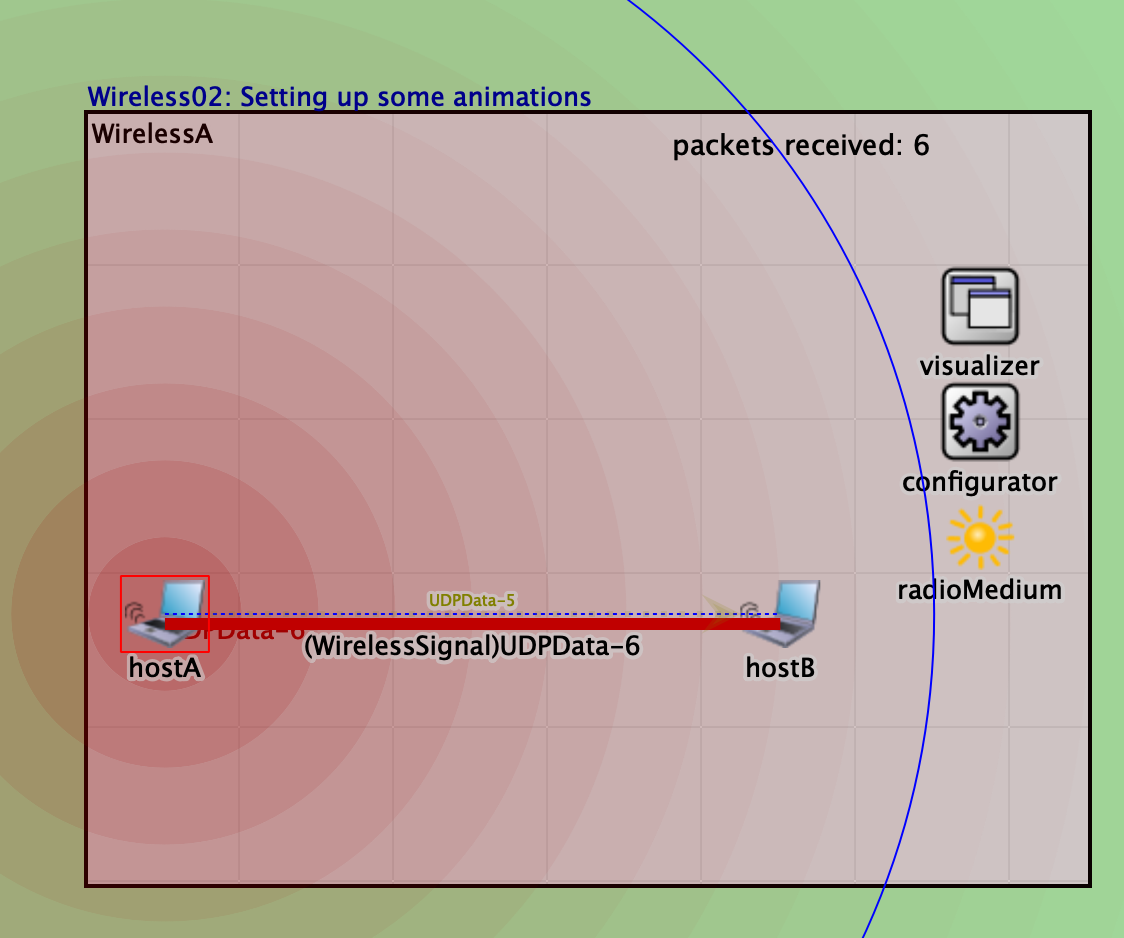
\includegraphics[keepaspectratio]{resources/transmission.png}}

}

\caption{\label{fig-transmission}Transmission Range}

\end{figure}%

Figure~\ref{fig-transmission} visualizes the radio transmission range,
showing the communication radius around \texttt{hostA}, represented by
the blue circle. The range is set to \texttt{500m} as specified in the
\texttt{omnetpp.ini} configuration file:

\begin{Shaded}
\begin{Highlighting}[]
\DataTypeTok{*.host*.wlan}\KeywordTok{[0]}\DataTypeTok{.radio.transmitter.\textbackslash{}}
\DataTypeTok{  communicationRange }\OtherTok{=}\StringTok{ 500m}
\end{Highlighting}
\end{Shaded}

\subsection{Change the communication range so that host B is no longer
reachable from host A. Visualize the new
range.}\label{change-the-communication-range-so-that-host-b-is-no-longer-reachable-from-host-a.-visualize-the-new-range.}

\begin{figure}

\centering{

\pandocbounded{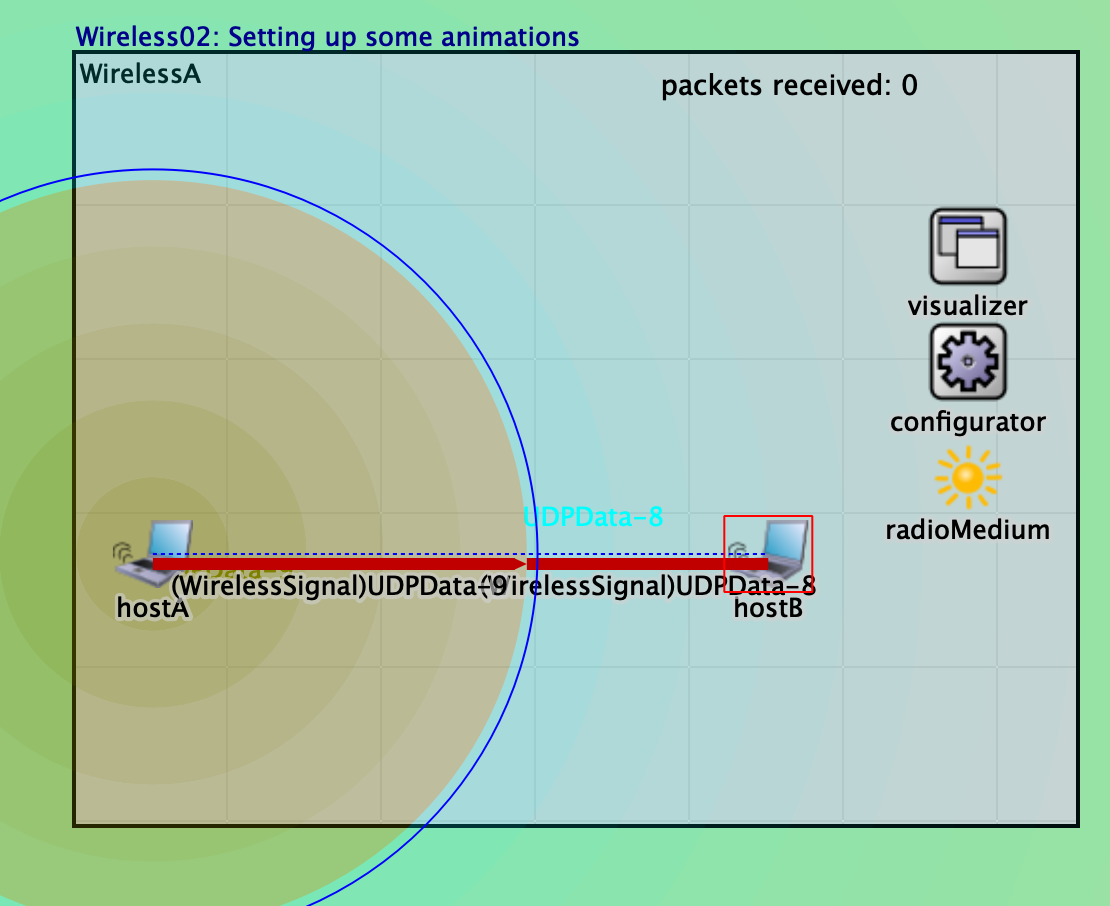
\includegraphics[keepaspectratio]{resources/transmission_reduced.png}}

}

\caption{\label{fig-transmission-reduced}Reduced Transmission Range}

\end{figure}%

Figure~\ref{fig-transmission-reduced} illustrates the reduced
communication range, where the blue circle around \texttt{hostA} no
longer reaches \texttt{hostB}. This change was achieved by modifying the
communication range parameter in the \texttt{omnetpp.ini} file:

\begin{Shaded}
\begin{Highlighting}[]
\DataTypeTok{*.host*.wlan}\KeywordTok{[0]}\DataTypeTok{.radio.transmitter.\textbackslash{}}
\DataTypeTok{  communicationRange }\OtherTok{=}\StringTok{ 250m}
\end{Highlighting}
\end{Shaded}

\subsection{Provide simulation results for the transmission rate and
explain
them.}\label{provide-simulation-results-for-the-transmission-rate-and-explain-them.}

To provide results, the range is set back to \texttt{500m} in the
\texttt{omnetpp.ini} file. The simulation is run and the following
output is generated:

\begin{Shaded}
\begin{Highlighting}[]
\NormalTok{Simulation time limit reached}
\NormalTok{  {-}{-} at t=20s, event \#21022}

\NormalTok{Radio signal}
\NormalTok{  arrival computation count = 1617}
\NormalTok{Transmission count = 1617}
\NormalTok{Signal send count = 1617}
\NormalTok{Reception computation count = 1617}

\NormalTok{WirelessA.hostB.app[0]:}
\NormalTok{  received 1617 packets}
\end{Highlighting}
\end{Shaded}

The transmission count is \texttt{1617} packets, which is the same as
the previous result (with \texttt{seed-set\ =\ 1337}). The animation
only visualizes the network topology and does not interfere with the
simulation logic.

Leaving the communication range at \texttt{250m} would result in
\texttt{hostB} being unreachable from \texttt{hostA}:

\begin{Shaded}
\begin{Highlighting}[]
\NormalTok{WirelessA.hostB.app[0]: received 0 packets}
\end{Highlighting}
\end{Shaded}

The output confirms that no packets were received from \texttt{hostB},
indicating that the reduced communication range successfully prevented
communication between the two hosts.

\section{Adding more nodes and decreasing the communication
range}\label{adding-more-nodes-and-decreasing-the-communication-range}

\subsection{Identify the type of wireless interfaces for the new hosts.
Explain your answer with references to the source
code.}\label{identify-the-type-of-wireless-interfaces-for-the-new-hosts.-explain-your-answer-with-references-to-the-source-code.}

The three new hosts (\texttt{hostR1}, \texttt{hostR2} and
\texttt{hostR3}) are defined in the \texttt{WirelessB.ned} network
configuration:

\begin{Shaded}
\begin{Highlighting}[]
\NormalTok{network WirelessB }\KeywordTok{extends}\NormalTok{ WirelessA}
\NormalTok{\{}
  \DataTypeTok{submodules}\OperatorTok{:}
    \DataTypeTok{hostR1}\OperatorTok{:} \OperatorTok{\textless{}}\ImportTok{default}\NormalTok{(}\StringTok{"WirelessHost"}\NormalTok{)}\OperatorTok{\textgreater{}}\NormalTok{\textbackslash{}}
\NormalTok{      like INetworkNode \{}
\NormalTok{        @}\FunctionTok{display}\NormalTok{(}\StringTok{"p=250,300"}\NormalTok{)}\OperatorTok{;}
\NormalTok{    \}}
    \DataTypeTok{hostR2}\OperatorTok{:} \OperatorTok{\textless{}}\ImportTok{default}\NormalTok{(}\StringTok{"WirelessHost"}\NormalTok{)}\OperatorTok{\textgreater{}}\NormalTok{\textbackslash{}}
\NormalTok{      like INetworkNode \{}
\NormalTok{        @}\FunctionTok{display}\NormalTok{(}\StringTok{"p=150,450"}\NormalTok{)}\OperatorTok{;}
\NormalTok{    \}}
    \DataTypeTok{hostR3}\OperatorTok{:} \OperatorTok{\textless{}}\ImportTok{default}\NormalTok{(}\StringTok{"WirelessHost"}\NormalTok{)}\OperatorTok{\textgreater{}}\NormalTok{\textbackslash{}}
\NormalTok{      like INetworkNode \{}
\NormalTok{        @}\FunctionTok{display}\NormalTok{(}\StringTok{"p=350,450"}\NormalTok{)}\OperatorTok{;}
\NormalTok{    \}}
\NormalTok{\}}
\end{Highlighting}
\end{Shaded}

The \texttt{WirelessHost} is defined in
\texttt{/node/inet/WirelessHost.ned}:

\begin{Shaded}
\begin{Highlighting}[]
\NormalTok{module WirelessHost }\KeywordTok{extends}\NormalTok{ StandardHost}
\NormalTok{\{}
    \DataTypeTok{parameters}\OperatorTok{:}
\NormalTok{        numWlanInterfaces }\OperatorTok{=} \ImportTok{default}\NormalTok{(}\DecValTok{1}\NormalTok{)}\OperatorTok{;}
\NormalTok{        @}\FunctionTok{display}\NormalTok{(}\StringTok{"i=device/wifilaptop"}\NormalTok{)}\OperatorTok{;}
\NormalTok{\}}
\end{Highlighting}
\end{Shaded}

``Models a host with (default) one wireless (802.11) card in
infrastructure mode'' (l. 11).

The wireless interfaces for these hosts are specified in the
\texttt{omnetpp.ini} file:

\begin{Shaded}
\begin{Highlighting}[]
\DataTypeTok{*.host*.wlan}\KeywordTok{[0]}\DataTypeTok{.typename }\OtherTok{=}\StringTok{\textbackslash{}}
\DataTypeTok{  "AckingWirelessInterface"}
\end{Highlighting}
\end{Shaded}

Again, the \texttt{AckingWirelessInterface} type is used for the
wireless interfaces of all hosts in the network.

\section{Setting up static routing}\label{setting-up-static-routing}

\subsection{Use the runtime GUI to capture a screenshot showing the IP
addresses of all hosts in the
network.}\label{use-the-runtime-gui-to-capture-a-screenshot-showing-the-ip-addresses-of-all-hosts-in-the-network.}

Set the following option in the \texttt{omnetpp.ini} file to enable this
debugging information:

\begin{Shaded}
\begin{Highlighting}[]
\DataTypeTok{INFO: hostA }\KeywordTok{[...]}
\DataTypeTok{  \{inet\_addr:10.0.0.1/24}\KeywordTok{[...]}\DataTypeTok{\}}
\DataTypeTok{INFO: hostB }\KeywordTok{[...]}
\DataTypeTok{  \{inet\_addr:10.0.0.2/24}\KeywordTok{[...]}\DataTypeTok{\}}
\DataTypeTok{INFO: hostR1 }\KeywordTok{[...]}
\DataTypeTok{  \{inet\_addr:10.0.0.3/24}\KeywordTok{[...]}\DataTypeTok{\}}
\DataTypeTok{INFO: hostR2 }\KeywordTok{[...]}
\DataTypeTok{  \{inet\_addr:10.0.0.4/24}\KeywordTok{[...]}\DataTypeTok{\}}
\DataTypeTok{INFO: hostR3 }\KeywordTok{[...]}
\DataTypeTok{  \{inet\_addr:10.0.0.5/24}\KeywordTok{[...]}\DataTypeTok{\}}
\end{Highlighting}
\end{Shaded}

Alternatively, the routing table can be viewed in the runtime GUI by
selecting the \texttt{hostA} module and clicking on
\texttt{Routing\ Table} in the \texttt{ipv4} section:

\begin{figure}

\centering{

\pandocbounded{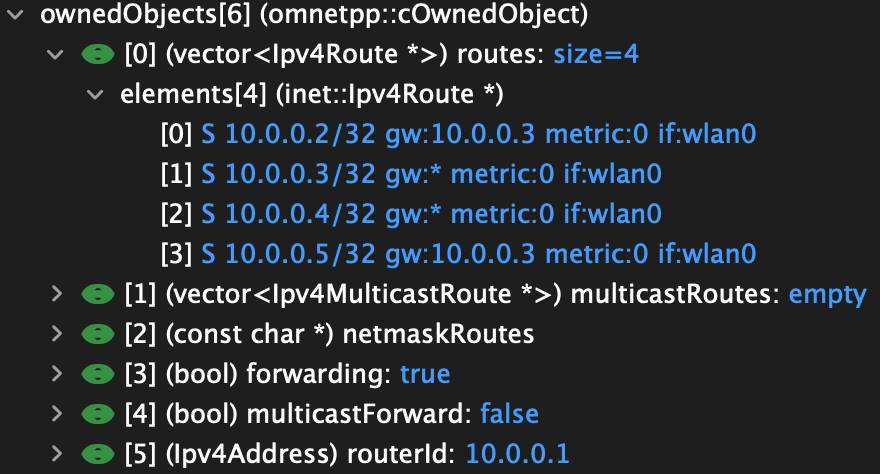
\includegraphics[keepaspectratio]{resources/routing_table.png}}

}

\caption{\label{fig-routing_table}Routing Table Host A}

\end{figure}%

Figure~\ref{fig-routing_table} displays the routing table for
\texttt{hostA}, showing the IP addresses of all hosts in the network.

\section{Taking interference into account}\label{sec-step_5}

\subsection{Enable event log recording in the runtime
GUI.}\label{enable-event-log-recording-in-the-runtime-gui.}

\begin{figure}

\centering{

\pandocbounded{
\includegraphics[keepaspectratio]{resources/event_logging.png}}

}

\caption{\label{fig-event_logging}Enable Event Logging}

\end{figure}%

Figure~\ref{fig-event_logging} shows that the ``Eventlog Recording''
option is enabled in the runtime GUI.

\subsection{\texorpdfstring{Open the \texttt{.elog} file with a text
editor and explain its
contents.}{Open the .elog file with a text editor and explain its contents.}}\label{open-the-.elog-file-with-a-text-editor-and-explain-its-contents.}

An excerpt from the \texttt{.elog} file is as follows:

\begin{Shaded}
\begin{Highlighting}[]
\NormalTok{CM id 243061 tid 243061 eid 243061}
\NormalTok{  etid 243061 c}
\NormalTok{    omnetpp::cMessage n UDPData{-}0 pe {-}1}
\NormalTok{BS id 243061 tid 243061 eid 243061}
\NormalTok{  etid 243061 c}
\NormalTok{    inet::Packet n}
\NormalTok{      UDPData{-}0 l 8000 m 54 pe 4}

\NormalTok{SH sm 54 sg 3}
\NormalTok{CMB sm 54 tm 55 m arrived}

\NormalTok{ES id 242948 tid 242948 eid 242948}
\NormalTok{  etid 242948 c}
\NormalTok{    inet::ClockEvent n}
\NormalTok{      sendTimer k 2 sm 54 st}
\NormalTok{        0.007276585767 am 54 at}
\NormalTok{          0.026732847636 pe 14}

\NormalTok{CMB sm 51 tm 25 m packetReceivedFromUpper}
\NormalTok{CME}
\NormalTok{CMB sm 51 tm 27 m packetReceivedFromUpper}
\NormalTok{CME}
\NormalTok{CMB sm 51 tm 30 m packetReceivedFromUpper}

\NormalTok{CMB sm 61 tm 4 m transmitPacket}
\NormalTok{BS id 242927 tid 242927 eid 242927}
\NormalTok{  etid 242927 c}
\NormalTok{    omnetpp::cMessage n}
\NormalTok{      removeNonInterferingTransmissions}
\NormalTok{        sm 4 st 0.002868038578}
\NormalTok{          am 4 at 0.021373372834}
\NormalTok{            pe 9}

\NormalTok{CMB sm 182 tm 30 m packetReceivedFromLower}
\NormalTok{CME}

\NormalTok{MDC id 74 d}
\NormalTok{  "t=processed 1 pk (1008 B);}
\NormalTok{    p=550,300;b=600,5,,,,1"}

\NormalTok{CMB sm 75 tm 69 m}
\NormalTok{  findBestMatchingRoute(10.0.0.2)}
\NormalTok{CME}
\NormalTok{CMB sm 75 tm 76 m}
\NormalTok{  resolveL3Address}
\NormalTok{CME}
\end{Highlighting}
\end{Shaded}

In general, the file captures the detailed sequence of events and
interactions between modules during the simulation. Key events include:

\begin{enumerate}
\def\labelenumi{\arabic{enumi}.}
\tightlist
\item
  \textbf{Message Creation:} A packet (\texttt{UDPData-0}) is created as
  an instance of \texttt{inet::Packet} with a size of \texttt{8000} bits
  and processed by submodules (\texttt{CM} and \texttt{BS} events).
\item
  \textbf{Signal Handling and Arrival:} Signals are processed by
  submodules (\texttt{SH} events) and packets arrive at target
  submodules (\texttt{CMB} events).
\item
  \textbf{Event Scheduling:} Timers and network events (\texttt{ES}) are
  scheduled for execution, such as the \texttt{sendTimer} for managing
  transmissions.
\item
  \textbf{Packet Processing and Transmission:} Packets are received from
  upper layers, processed and transmitted at various stages
  (\texttt{CMB} with \texttt{packetReceivedFromUpper} and
  \texttt{transmitPacket}).
\item
  \textbf{Address Resolution:} Submodules resolve layer 3 addresses and
  identify routes (\texttt{CMB} \texttt{findBestMatchingRoute}).
\item
  \textbf{Visualization Updates:} Visualization logs (\texttt{MDC}) show
  processed packets and their visual representation on the simulation
  canvas.
\end{enumerate}

This information provides a comprehensive view of packet flow and module
interactions that can be used to analyze system behavior and
performance.

\subsection{\texorpdfstring{Analyze the event log using the sequence
chart and event log table tools. Filter events for \texttt{hostA+udp},
\texttt{hostB+udp} and
\texttt{hostR1+ip}.}{Analyze the event log using the sequence chart and event log table tools. Filter events for hostA+udp, hostB+udp and hostR1+ip.}}\label{analyze-the-event-log-using-the-sequence-chart-and-event-log-table-tools.-filter-events-for-hostaudp-hostbudp-and-hostr1ip.}

\begin{figure}

\centering{

\pandocbounded{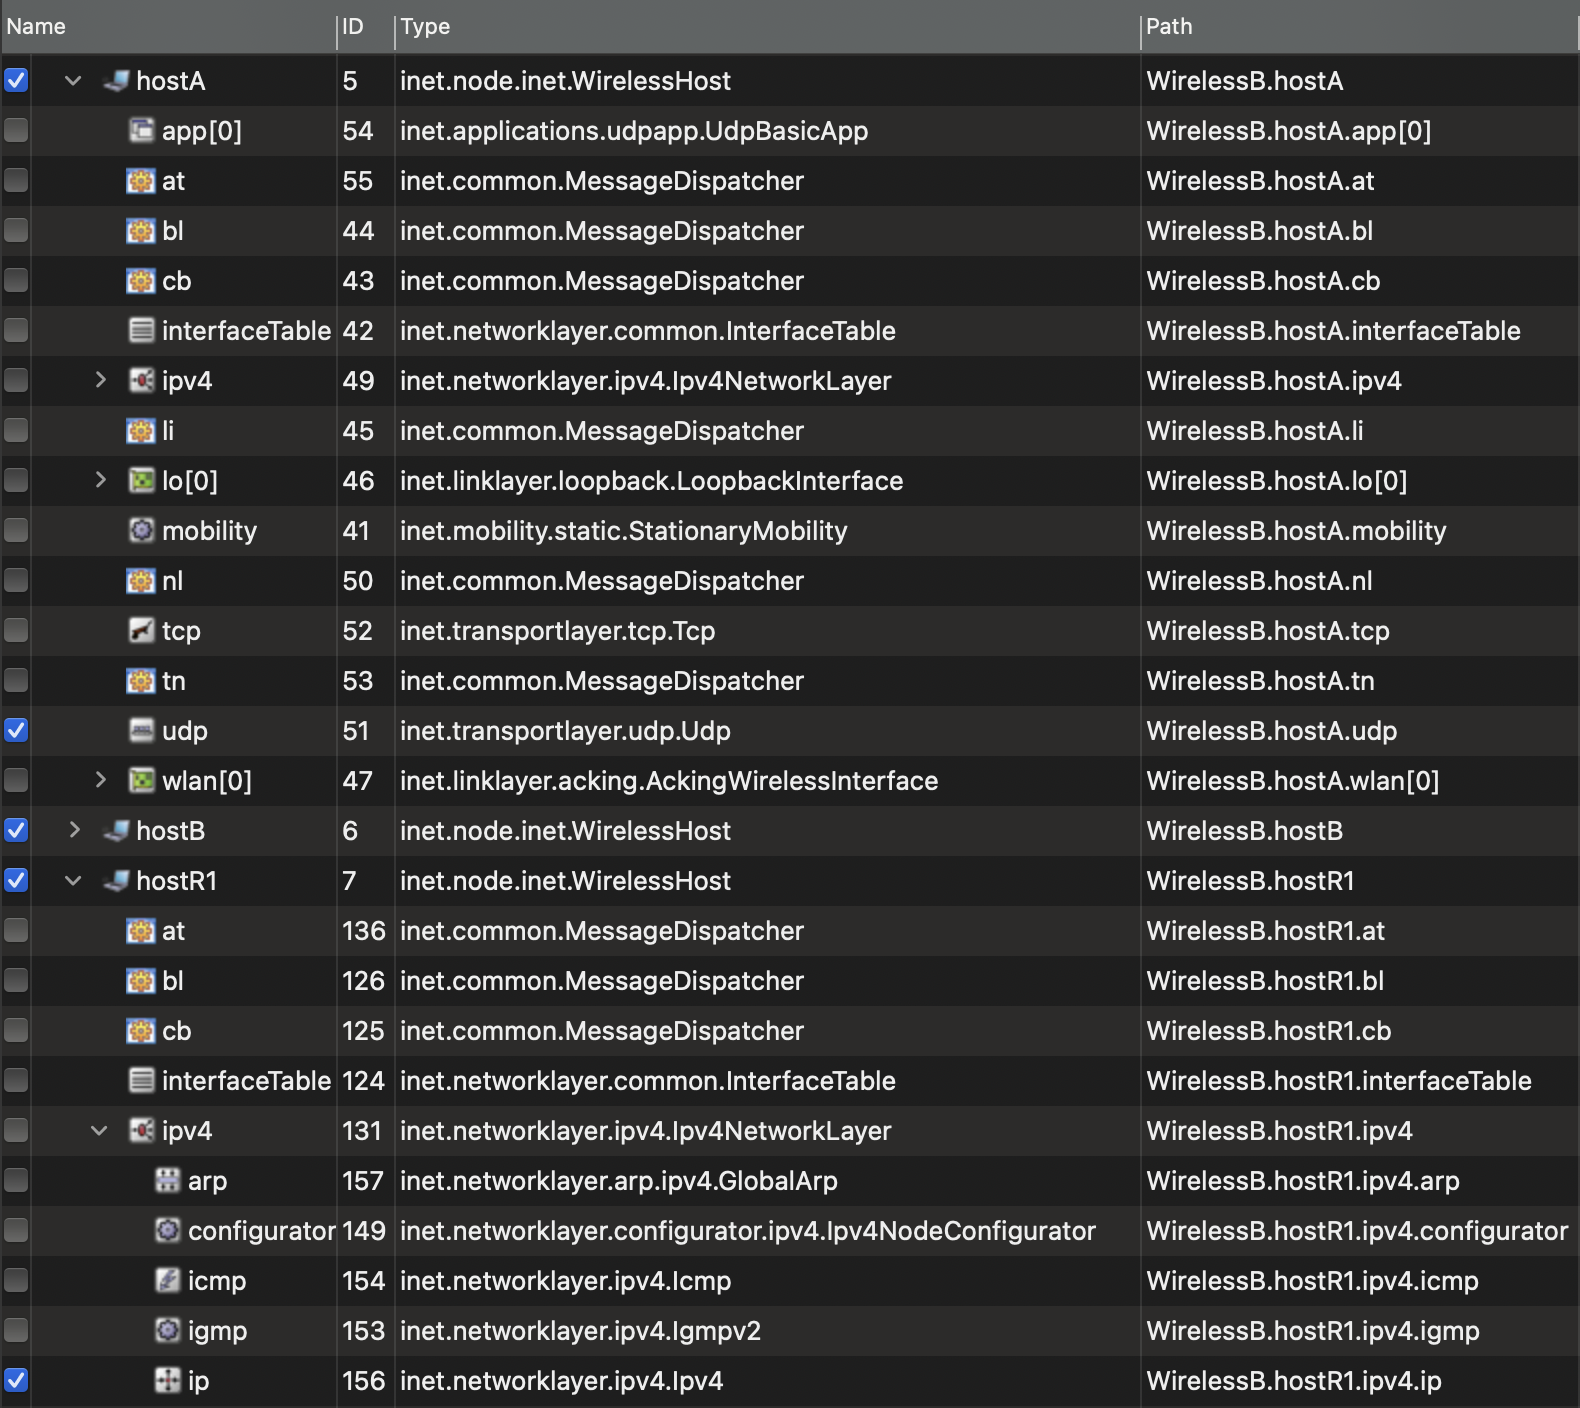
\includegraphics[keepaspectratio]{resources/filter_event_log.png}}

}

\caption{\label{fig-filter_event_log}Filter Event Log}

\end{figure}%

Figure~\ref{fig-filter_event_log} shows the event log filtering options
for \texttt{hostA+udp}, \texttt{hostB+udp} and \texttt{hostR1+ip} in the
runtime GUI.

\subsection{Take screenshots and comment on both a complete and an
incomplete transmission sequence
chart.}\label{take-screenshots-and-comment-on-both-a-complete-and-an-incomplete-transmission-sequence-chart.}

\begin{figure}

\centering{

\pandocbounded{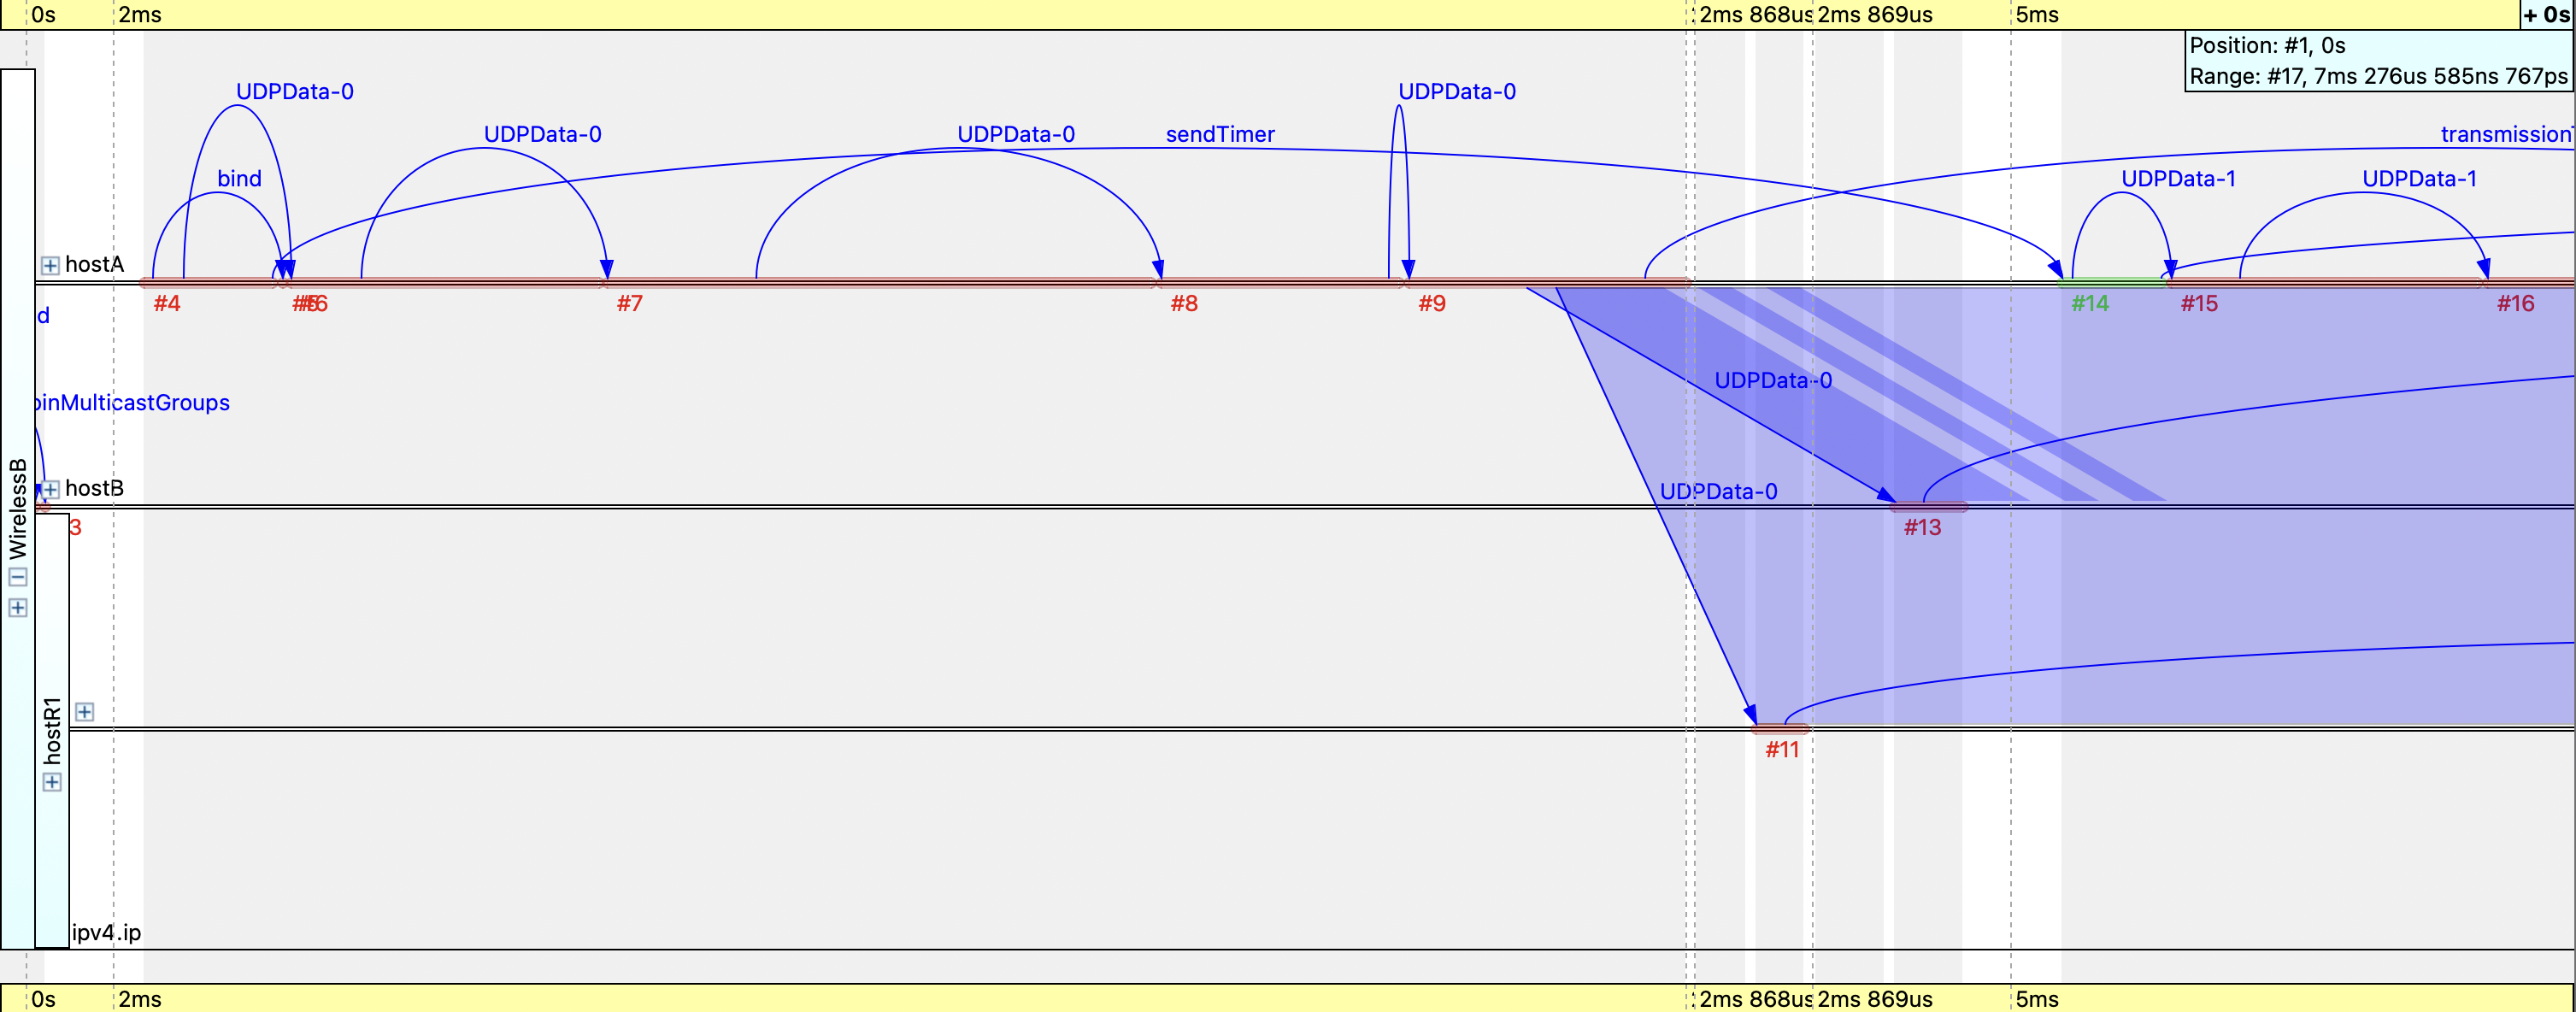
\includegraphics[keepaspectratio]{resources/elog_0.png}}

}

\caption{\label{fig-event_log_start}Event Log Start}

\end{figure}%

Figure~\ref{fig-event_log_start} shows the first events of the
simulation. At \texttt{Event\ \#4} it starts with the \texttt{bind}
operation for \texttt{UDPData-0} in \texttt{hostA}. This step represents
the initialization of the UDP communication, including the creation of
the packet and its preparation for transmission. At this point, the
\texttt{UDPData-0} message is scheduled for delivery, marking the start
of its journey from \texttt{hostA}.

The illustration is further simplified by using the \emph{Network
Interface} option in the \emph{Preset Configuration}:

\begin{figure}

\centering{

\pandocbounded{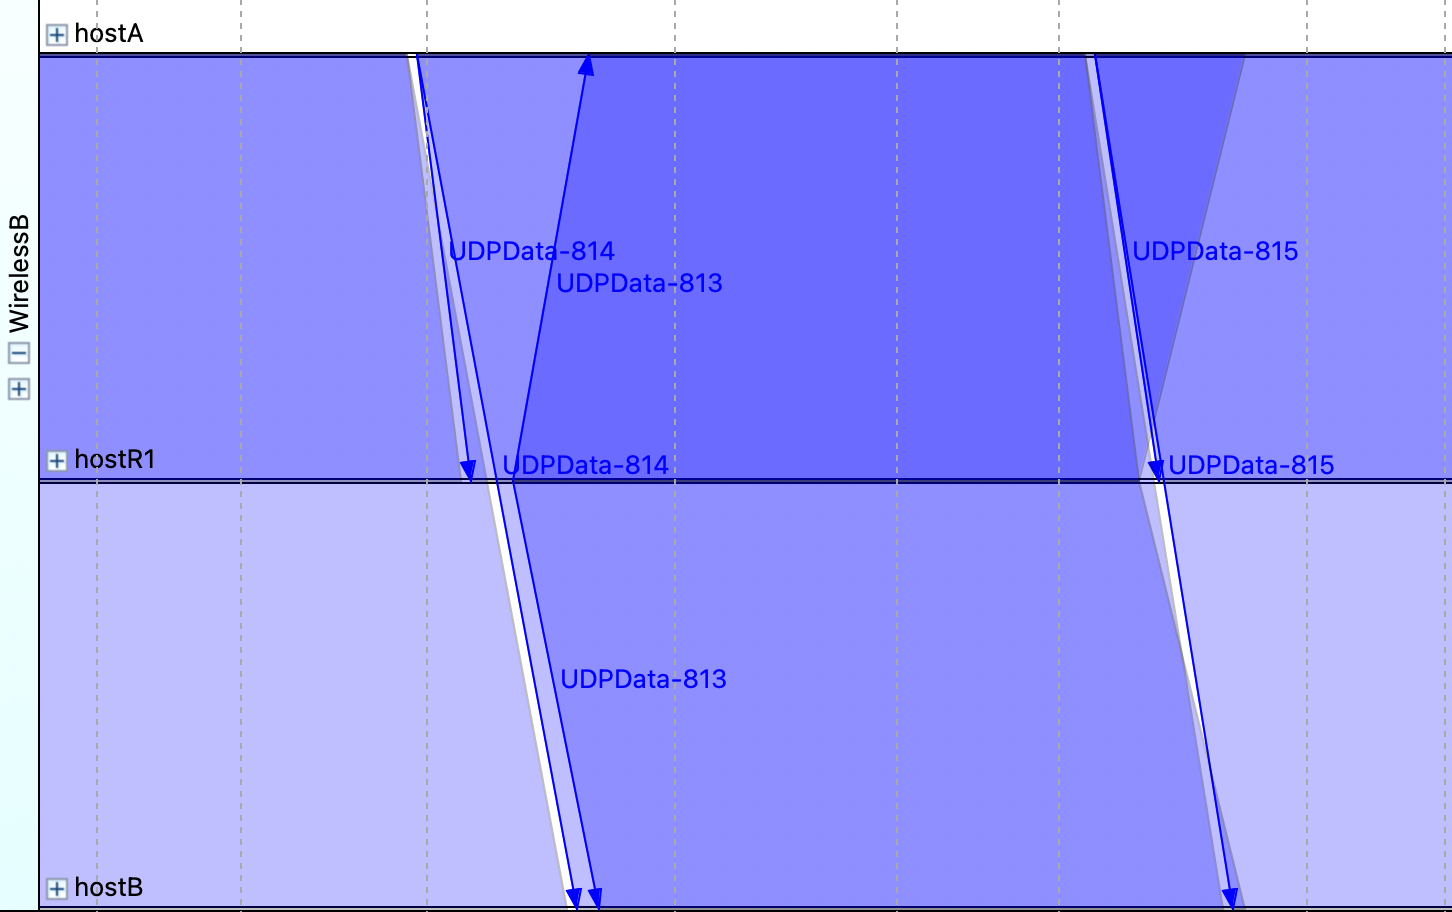
\includegraphics[keepaspectratio]{resources/elog_events.png}}

}

\caption{\label{fig-event_log_events}Event Log Simplified}

\end{figure}%

As shown in Figure~\ref{fig-event_log_events}, the sequence chart shows
the status of three packets (\texttt{UDPData-813}, \texttt{UDPData-814}
and \texttt{UDPData-815}):

\begin{itemize}
\tightlist
\item
  \textbf{\texttt{UDPData-813}:} Successfully reaches \texttt{hostB}
  after being forwarded by \texttt{hostR1}. The arcs indicate a complete
  flow from \texttt{hostA} to \texttt{hostB} via \texttt{hostR1}.
\item
  \textbf{\texttt{UDPData-814}:} Is transmitted from \texttt{hostA} to
  \texttt{hostR1} but does not reach \texttt{hostB}. The absence of arcs
  from \texttt{hostR1} to \texttt{hostB} indicates that the packet was
  either dropped or lost.
\item
  \textbf{\texttt{UDPData-815}:} Also fails to reach \texttt{hostB}
  after being sent to \texttt{hostR1}. Similar to \texttt{UDPData-814},
  the packet appears to have been dropped or interrupted before reaching
  its final destination.
\end{itemize}

This simplified view highlights the occurrence of packet loss or
forwarding problems at \texttt{hostR1}, indicating the need for further
analysis of routing or congestion effects on the network.

\section{Using CSMA to better utilize the medium}\label{sec-step_6}

\subsection{\texorpdfstring{1. Compare the number of packets received by
host B in this configuration with the results from \emph{Configuration
Step 5} (Section~\ref{sec-step_5}). Explain the
difference.}{1. Compare the number of packets received by host B in this configuration with the results from Configuration Step 5 (Section~). Explain the difference.}}\label{compare-the-number-of-packets-received-by-host-b-in-this-configuration-with-the-results-from-configuration-step-5-sec-step_5.-explain-the-difference.}

Running the simulation with the CSMA configuration produces the
following output:

\begin{Shaded}
\begin{Highlighting}[]
\NormalTok{WirelessB.hostB.app[0]:}
\NormalTok{  received 1090 packets}
\end{Highlighting}
\end{Shaded}

In Section~\ref{sec-step_5} it was:

\begin{Shaded}
\begin{Highlighting}[]
\NormalTok{WirelessB.hostB.app[0]:}
\NormalTok{  received 139 packets}
\end{Highlighting}
\end{Shaded}

The number of packets received by \texttt{hostB} in this configuration
is \texttt{1090}, which is significantly higher than the \texttt{139}
packets received in the previous configuration. This difference can be
attributed to the use of CSMA in the current configuration, which allows
for better utilization of the medium by coordinating access to the
channel among multiple nodes. The CSMA protocol helps reduce collisions
and interference, resulting in more successful packet transmissions and
higher throughput compared to the previous configuration.

\section{Turning on ACKs in CSMA}\label{sec-step_7}

\subsection{\texorpdfstring{Measure the \texttt{numRetry} statistic for
\emph{Configuration Steps 6} (Section~\ref{sec-step_6}) and
\emph{7}.}{Measure the numRetry statistic for Configuration Steps 6 (Section~) and 7.}}\label{measure-the-numretry-statistic-for-configuration-steps-6-sec-step_6-and-7.}

The \texttt{numRetry} statistic is measured in the simulation output
(\texttt{Wireless06.sca}):

\begin{Shaded}
\begin{Highlighting}[]
\NormalTok{scalar WirelessB.hostA.wlan[0].mac}
\NormalTok{  numRetry 0}
\NormalTok{scalar WirelessB.hostB.wlan[0].mac}
\NormalTok{  numRetry 0}
\NormalTok{scalar WirelessB.hostR1.wlan[0].mac}
\NormalTok{  numRetry 0}
\NormalTok{scalar WirelessB.hostR2.wlan[0].mac}
\NormalTok{  numRetry 0}
\NormalTok{scalar WirelessB.hostR3.wlan[0].mac}
\NormalTok{  numRetry 0}
\end{Highlighting}
\end{Shaded}

and (\texttt{Wireless07.sca}):

\begin{Shaded}
\begin{Highlighting}[]
\NormalTok{scalar WirelessB.hostA.wlan[0].mac}
\NormalTok{  numRetry 67}
\NormalTok{scalar WirelessB.hostB.wlan[0].mac}
\NormalTok{  numRetry 0}
\NormalTok{scalar WirelessB.hostR1.wlan[0].mac}
\NormalTok{  numRetry 67}
\NormalTok{scalar WirelessB.hostR2.wlan[0].mac}
\NormalTok{  numRetry 0}
\NormalTok{scalar WirelessB.hostR3.wlan[0].mac}
\NormalTok{  numRetry 0}
\end{Highlighting}
\end{Shaded}

\subsection{\texorpdfstring{Cite the source code where the logic for
\texttt{numRetry} is
defined.}{Cite the source code where the logic for numRetry is defined.}}\label{cite-the-source-code-where-the-logic-for-numretry-is-defined.}

The logic for \texttt{numRetry} is implemented in
\texttt{inet/linklayer/csmaca/CsmaCaMac.cc}:

\begin{Shaded}
\begin{Highlighting}[]
\NormalTok{numRetry }\OperatorTok{=} \DecValTok{0}\OperatorTok{;}
\NormalTok{WATCH}\OperatorTok{(}\NormalTok{numRetry}\OperatorTok{);}

\DataTypeTok{void}\NormalTok{ CsmaCaMac}\OperatorTok{::}\NormalTok{finish}\OperatorTok{()}
\OperatorTok{\{}
\NormalTok{    recordScalar}\OperatorTok{(}\StringTok{"numRetry"}\OperatorTok{,}\NormalTok{ numRetry}\OperatorTok{);}
    \OperatorTok{...}
\OperatorTok{\}}

\DataTypeTok{void}\NormalTok{ CsmaCaMac}\OperatorTok{::}\NormalTok{retryCurrentTransmission}\OperatorTok{()}
\OperatorTok{\{}
\NormalTok{    ASSERT}\OperatorTok{(}\NormalTok{retryCounter }\OperatorTok{\textless{}}\NormalTok{ retryLimit}\OperatorTok{);}
\NormalTok{    retryCounter}\OperatorTok{++;}
\NormalTok{    numRetry}\OperatorTok{++;}
\NormalTok{    generateBackoffPeriod}\OperatorTok{();}
\OperatorTok{\}}
\end{Highlighting}
\end{Shaded}

At the start it is initialized with \texttt{0} and tracked using
\texttt{WATCH}. In the \texttt{finish()} method, \texttt{numRetry} is
recorded as a scalar statistic using \texttt{recordScalar()}. Each time
a packet is not successfully transmitted and a retry is initiated, the
\texttt{retryCurrentTransmission()} method increments \texttt{numRetry}.

\subsection{Explain the differences in this metric between the two
configurations.}\label{explain-the-differences-in-this-metric-between-the-two-configurations.}

The \texttt{numRetry} metric for \texttt{Configuration\ Step\ 6} is
\texttt{0} for all hosts because of the lack of ACKs. In
\texttt{Configuration\ Step\ 7}, the \texttt{numRetry} statistic is
\texttt{67} for \texttt{hostA} and \texttt{hostR1}, indicating the
number of retransmissions due to failed packet delivery attempts. The
increase in \texttt{numRetry} when ACKs are enabled is due to the
acknowledgment mechanism requiring retries when packets are lost or ACKs
are not received. While this increases the reliability of the network,
it also results in higher retransmission counts, especially in scenarios
with higher traffic or interference.

\section{Configuring node movements}\label{configuring-node-movements}

\subsection{\texorpdfstring{Plot the \texttt{throughput\ vector} at
\texttt{hostB} and identify the time when the transmission
stops.}{Plot the throughput vector at hostB and identify the time when the transmission stops.}}\label{plot-the-throughput-vector-at-hostb-and-identify-the-time-when-the-transmission-stops.}

The following plot is generated using the \emph{Line Chart with
Matplotlib} tool in the runtime GUI:

\begin{figure}

\centering{

\pandocbounded{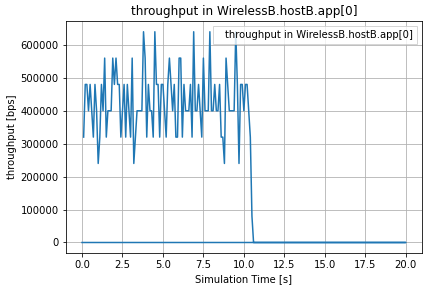
\includegraphics[keepaspectratio]{resources/throughput.png}}

}

\caption{\label{fig-throughput_vector}Throughput Vector Host B}

\end{figure}%

Figure~\ref{fig-throughput_vector} shows the \texttt{throughput\ vector}
at \texttt{hostB} over time. Transmission stops at about
\texttt{t=10.5s}, as indicated by the sharp drop in throughput to
\texttt{0\ bps}. This corresponds to the moment in the simulation when
\texttt{hostR1} leaves the communication range of \texttt{hostA},
leading to the termination of packet transmission.

\begin{figure}

\centering{

\pandocbounded{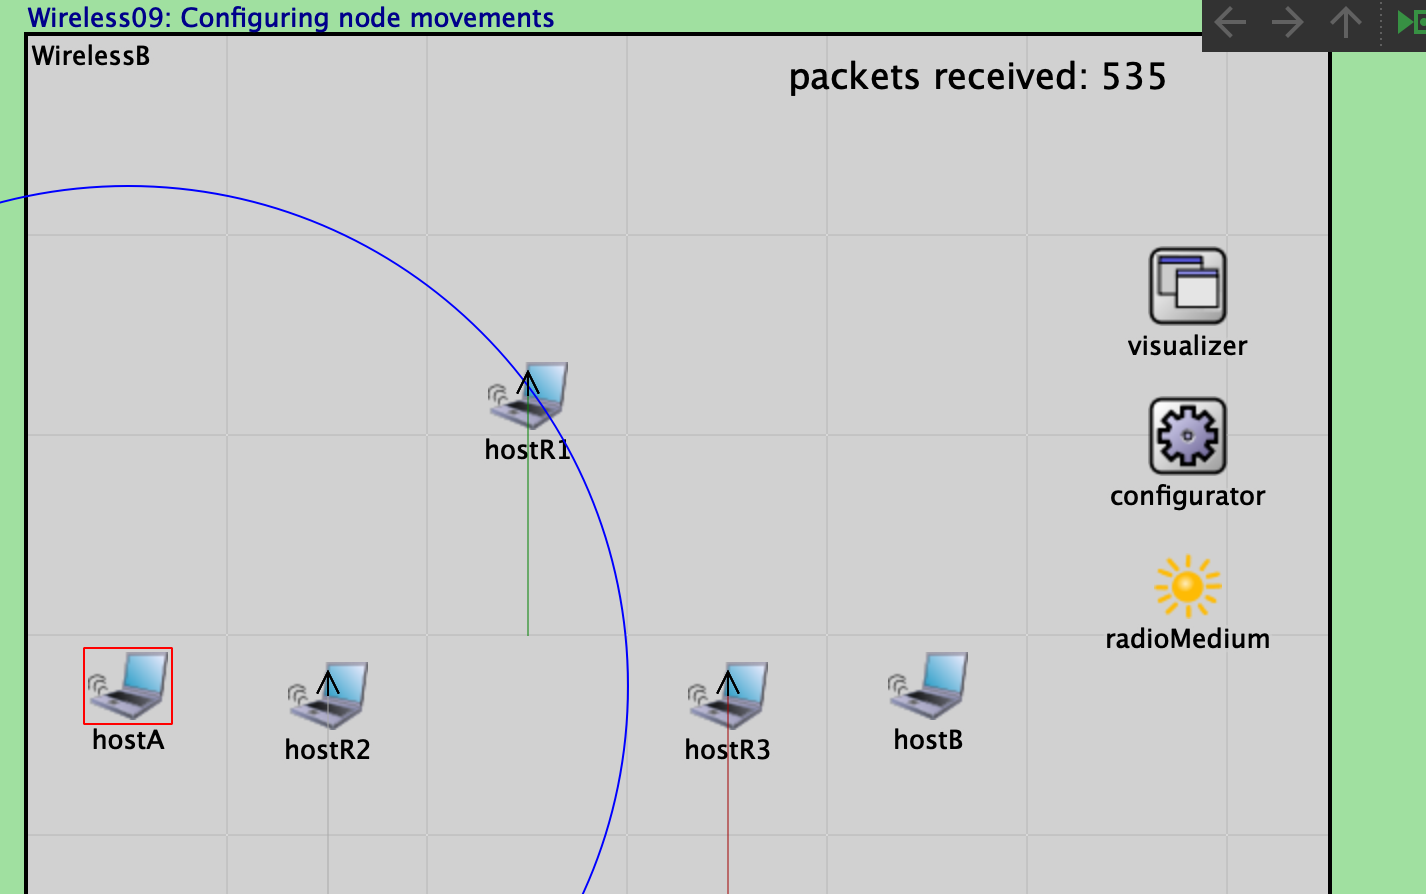
\includegraphics[keepaspectratio]{resources/t_10.png}}

}

\caption{\label{fig-simulation_t10}Simulation at t=10}

\end{figure}%

Figure~\ref{fig-simulation_t10} shows the simulation at \texttt{t=10s},
where the nodes have moved to new positions. Here, \texttt{hostR1} is
barely within the communication range of \texttt{hostA}, leading to the
resulting reduction in throughput and eventual termination of
transmissions.

\begin{figure}

\centering{

\pandocbounded{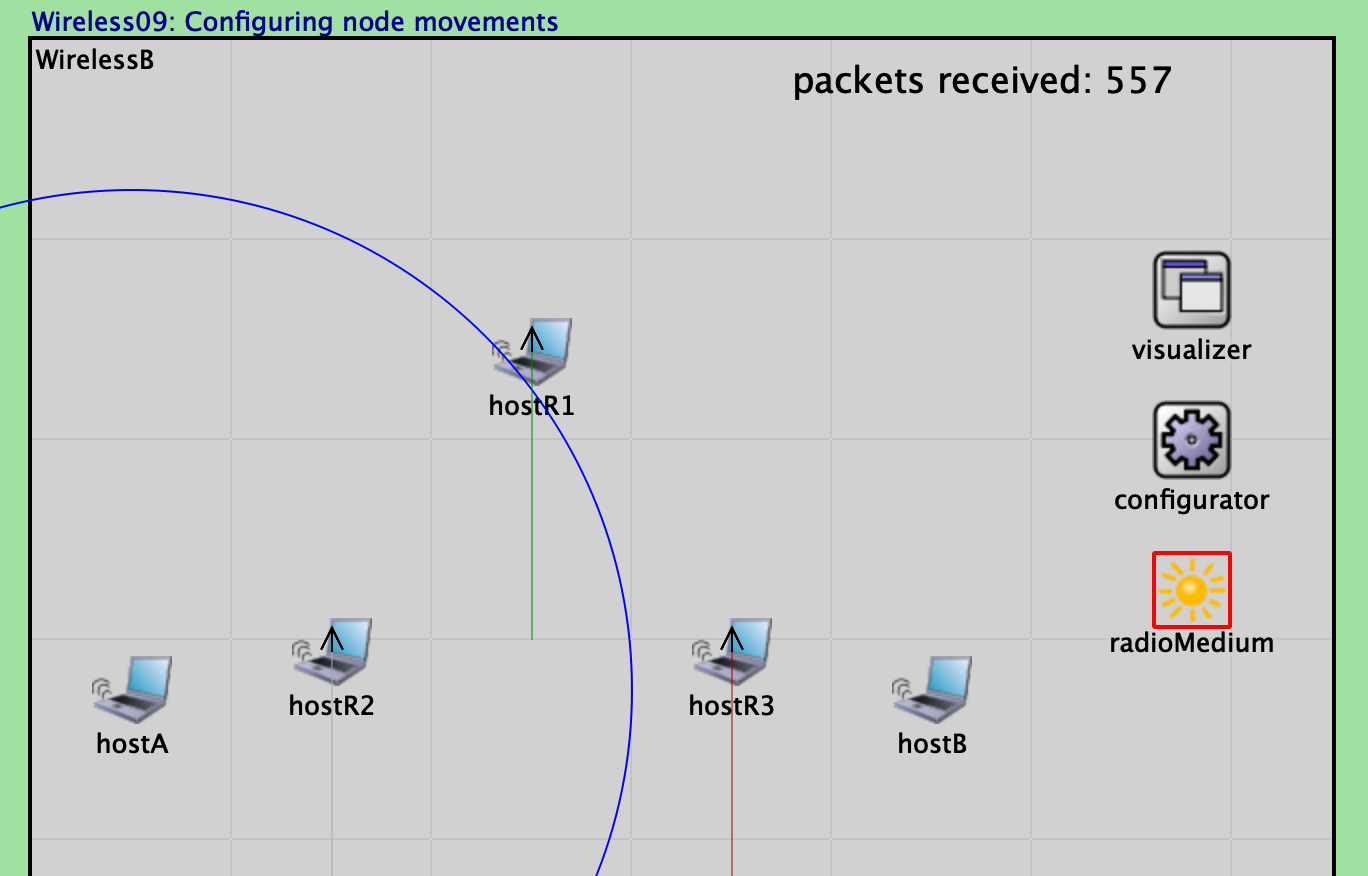
\includegraphics[keepaspectratio]{resources/t_12.png}}

}

\caption{\label{fig-simulation_t12}Simulation at t=12}

\end{figure}%

Figure~\ref{fig-simulation_t12} shows the simulation at \texttt{t=12s},
where \texttt{hostR1} has moved further away from \texttt{hostA},
resulting in complete loss of communication and termination of packet
transmission. A total of \texttt{557} packets were received by
\texttt{hostB} before the transmission stopped.

\section{Conclusion}\label{conclusion}

The wireless network simulations performed in this project demonstrate
the effectiveness of OMNeT++ and the INET framework in modeling complex
network scenarios. Key findings include the importance of proper
protocol configuration, such as enabling acknowledgment mechanisms in
CSMA, to ensure reliability despite the increased retransmission
overhead. Throughput measurements and event log analysis revealed the
impact of communication range, interference and mobility on network
performance. In addition, static and dynamic routing configurations were
successfully implemented and visualized, providing a clear understanding
of node interactions. Overall, the project highlights the versatility
and utility of simulation tools for studying wireless network behavior
and optimizing protocol design.

\section{References}\label{references}

\phantomsection\label{refs}
\begin{CSLReferences}{1}{0}
\bibitem[\citeproctext]{ref-inet2024}
INET Framework. n.d.a. {``{INET Framework}.''} Accessed January 14,
2025. \url{https://inet.omnetpp.org}.

\bibitem[\citeproctext]{ref-inet_wireless_tutorial2024}
---------. n.d.b. {``{INET Framework - Wireless Tutorial}.''} Accessed
January 14, 2025.
\url{https://inet.omnetpp.org/docs/tutorials/wireless/doc/index.html}.

\bibitem[\citeproctext]{ref-omnetpp2024}
OMNeT++. n.d.a. {``{OMNeT++}.''} Accessed January 14, 2025.
\url{https://omnetpp.org}.

\bibitem[\citeproctext]{ref-opp_env2024}
---------. n.d.b. {``{OMNeT++ Environment}.''} Accessed January 14,
2025. \url{https://omnetpp.org/opp_env}.

\end{CSLReferences}




\end{document}
